\documentclass[border=10pt]{standalone}

\usepackage{tikz}
\usepackage{tikzsymbols}
\usetikzlibrary{calc,patterns,shapes.geometric}

\def\centerarc[#1](#2)(#3:#4:#5){\draw[#1] ($(#2)+({#5*cos(#3)},{#5*sin(#3)})$) arc (#3:#4:#5);}

\begin{document}
	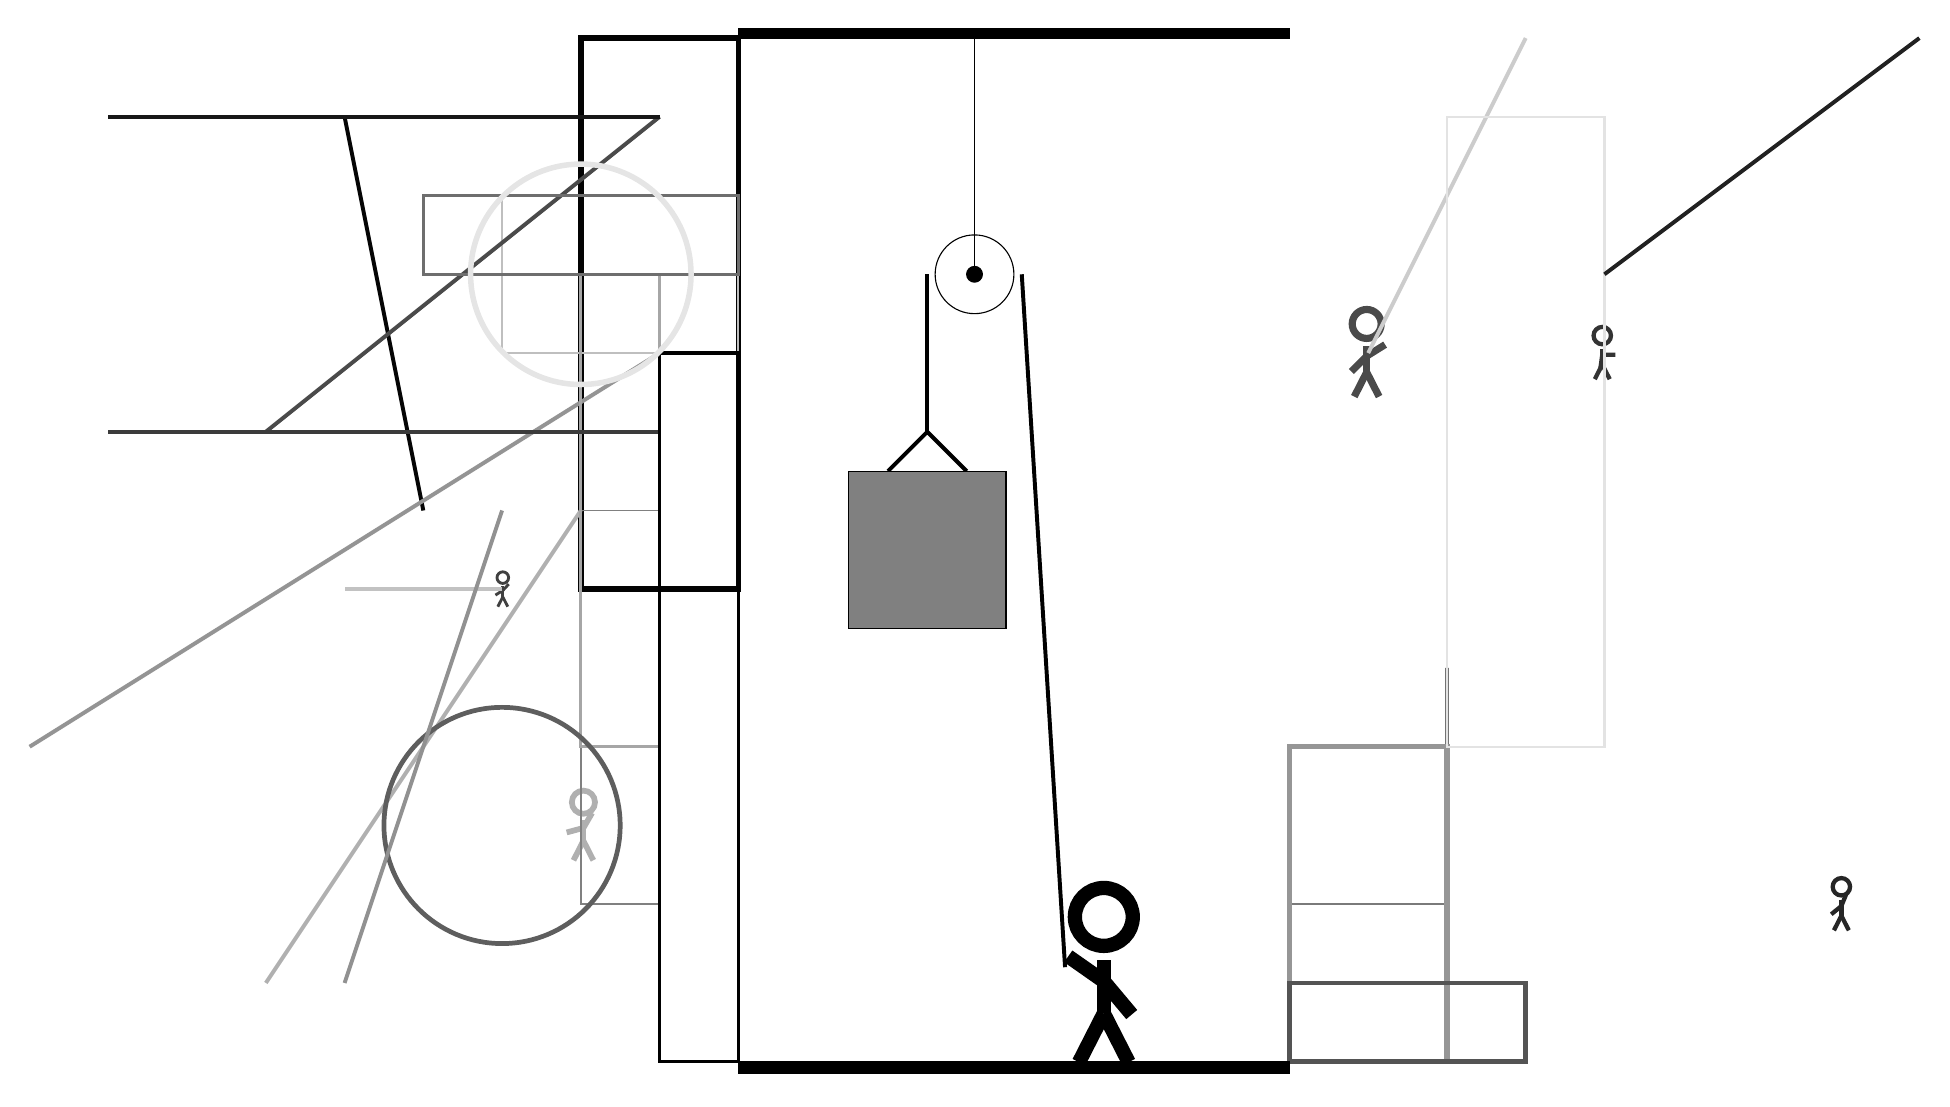
\begin{tikzpicture}
		%%%%% START %%%%%
		
		\draw[fill=black] (-2, 10) rectangle (5, 10.125);
		
		\draw (1, 7) circle (0.5);
		\draw[fill=black] (1, 7) circle (0.1);
		\draw (1, 10) -- (1, 7);
		
		\draw[line width=0.5mm] (-0.1, 4.5) -- (0.4, 5.0) -- (0.9, 4.5);
		\draw[fill=black!50] (-0.6, 4.5) rectangle (1.4, 2.5);
		
		\draw[line width=0.5mm] (0.4, 7) -- (0.4, 5.0);
		\centerarc[line width=0.5mm](1, 7)(0:180:0.6);
		\draw[line width=0.5mm](1.6, 7) -- (2.15, -1.8);
		
		\draw[line width=0.6mm, color=black!55] (7, 2) rectangle (7, -3);
		
		\draw[line width=0.7mm, color=black!99] (-4, 10) rectangle (-2, 3);
		\draw[line width=0.5mm, color=black!31](-4, 4) -- (-8, -2);
		\node[line width=0.5mm, color=black!71] at (6, 6) {\Strichmaxerl[5][45][32]};
		\node[line width=0.7mm, color=black!31] at (-4, 0) {\Strichmaxerl[4][15][60]};
		\draw[line width=0.2mm, color=black!52] (7, -1) rectangle (5, -1);
		
		\draw[line width=0.2mm, color=black!50] (-4, -1) rectangle (-3, 4);
		
		\draw[line width=0.7mm, color=black!41] (5, 1) rectangle (7, -3);
		\draw[line width=0.5mm, color=black!98](-7, 9) -- (-6, 4);
		\node[line width=0.6mm, color=black!80] at (9, 6) {\Strichmaxerl[3][82][1]};
		\draw[line width=0.6mm, color=black!67] (5, -3) rectangle (8, -2);
		\node[line width=0.7mm, color=black!75] at (-5, 3) {\Strichmaxerl[2][32][47]};
		\draw[line width=0.3mm, color=black!25] (-2, 6) rectangle (-5, 8);
		
		\draw[line width=0.5mm, color=black!71](-3, 9) -- (-8, 5);
		\draw[line width=0.5mm, color=black!42](-3, 6) -- (-11, 1);
		\draw[line width=0.4mm, color=black!35] (-3, 7) rectangle (-4, 1);
		\draw[line width=0.5mm, color=black!77](-3, 5) -- (-10, 5);
		\draw[line width=0.4mm, color=black!57] (-2, 7) rectangle (-6, 8);
		\draw[line width=0.5mm, color=black!24](-5, 3) -- (-7, 3);
		\draw[line width=0.5mm, color=black!20](6, 6) -- (8, 10);
		\draw[line width=0.5mm, color=black!91](-3, 9) -- (-10, 9);
		
		\draw[line width=0.3mm, color=black!11] (7, 1) rectangle (9, 9);
		
		\draw [line width=0.6mm, color=black!63](-5, 0) circle (1.5);
		\draw[line width=0.5mm, color=black!43](-5, 4) -- (-7, -2);
		\draw[line width=0.4mm, color=black!100] (-3, 6) rectangle (-2, -3);
		
		\draw[line width=0.5mm, color=black!87](9, 7) -- (13, 10);
		
		\draw [line width=0.7mm, color=black!10](-4, 7) circle (1.4);
		\node[line width=0.5mm, color=black!85] at (12, -1) {\Strichmaxerl[3][39][68]};
		
		\node at (2.6, -1.9) {\Strichmaxerl[10][-35][-50]};
		
		\draw[fill=black] (-2, -3) rectangle (5, -3.15);
		
		%%%%% END %%%%%
	\end{tikzpicture}
\end{document}